\section{Connecting Components (Jakub Jędrzejczyk)}

The functionality of allowing components to be connected together is handled by a dedicated blueprint actor, the \lstinline[language=C]|ComponentSlot|.
It is placed as a child actor within the components that are designed to have other components connected to them (e.g. the Motherboard has multiple slots for RAM sticks, a CPU socket, and PCIe slots for GPUs and other expansion cards) and represents a singular point of potential connection with another component.
They base \lstinline[language=C]|ComponentSlot| features a red cuboid using a similar material as the overlay material used for highlighting objects, making it transparent, yet visually distinct.

\begin{figure}[H]
	\centering
		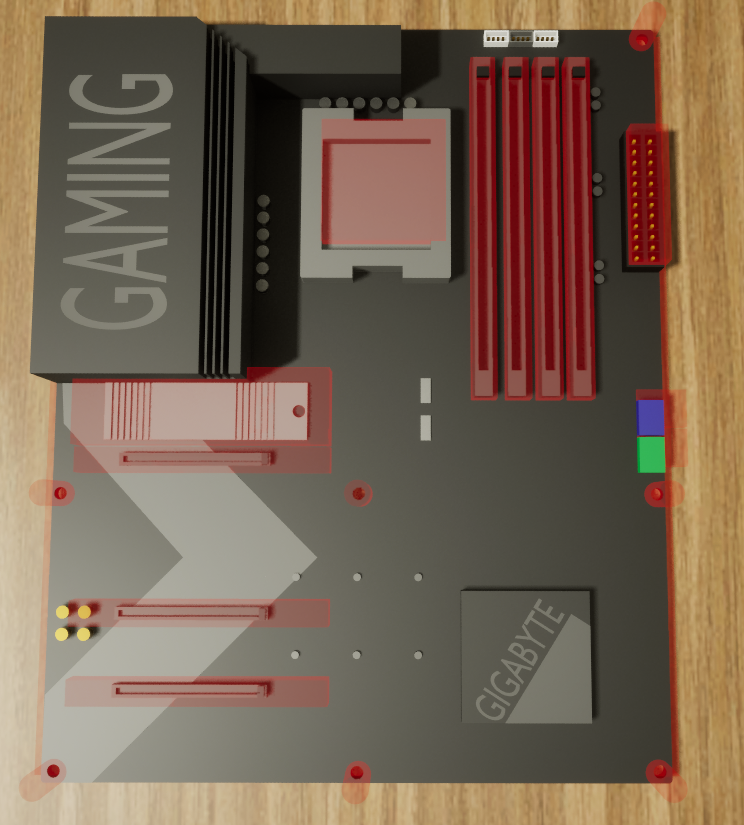
\includegraphics[width=0.6\textwidth]{Images/MotherboardWithSlots.png}
	\caption{Motherboard actor with visible ComponentSlot child actors.}
	\label{fig:MotherboardWithSlots}
\end{figure}

A number of them can be placed within a single component, as per figure \ref{fig:MotherboardWithSlots}, always scaled to appropriately cover the area where another component is expected to be connected.

Similarly to how the \lstinline[language=C]|Hand| actor handles highlighting objects, slots also use overlap events to detect collision and possibly begin the connection process.
On overlap with another component, the slot does a series of checks (see fig. \ref{fig:ComponentSlotBlueprintPreliminary}) to ensure the other actor:

\begin{itemize}
    \item is also a ComponentSlot; 
    \item that it's designed for the same component;
    \item that their type matches (so that, for example, a DDR5 RAM stick can not connect to a DDR4 slot);
    \item that the contacts (male or female) are not the same (so that e.g. two CPUs cannot be connected together);
    \item that neither of the two ComponentSlots is already occupied, i.e. in use for another connection;
    \item and (using the \lstinline[language=C]|AreSlotsCloseEnough()| function) that the two slots' rotation is within acceptable limits (up to 15 degrees of difference) for connection.
\end{itemize}

While the \lstinline[language=C]|AreSlotsCloseEnough()| function was originally used to ensure more accurate connection points by also checking the distance between ComponentSlots, this functionality was later deemed to be unnecessary, as the slots themselves can have their size modified to adjust the desired margins.

\begin{figure}[H]
	\centering
		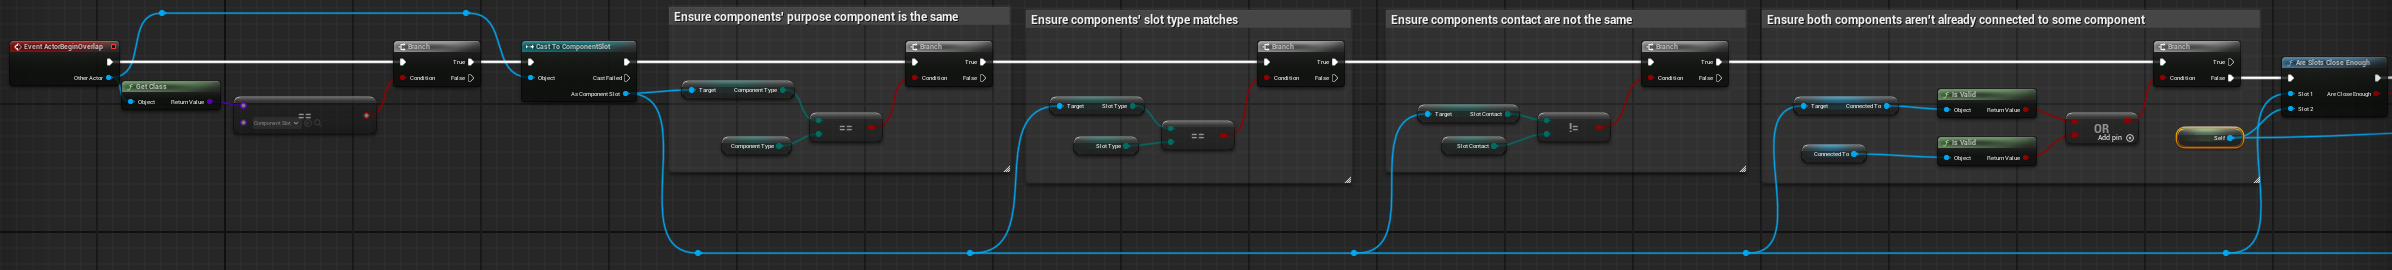
\includegraphics[width=1.0\textwidth]{Images/ComponentSlotBlueprintPreliminary.png}
	\caption{ComponentSlot's preliminary connection checks.}
	\label{fig:ComponentSlotBlueprintPreliminary}
\end{figure}

To ensure the connection process only ever happens after a component has been released from the hand, assuming the checks have passed, the slot makes use of event binding \cite{BindingUnbindingEvents} to listen for the \lstinline[language=C]|ObjectChangeHeldState| event from either of the two ComponentSlots' parent components, and launching the \lstinline[language=C]|EitherIntersectingObjectReleased| event.
To do so, two separate bindings are created, one for each of the two components involved in the potential connection.

While it may seem redundant to create these two bindings, it's important to note that because of the abstraction of the ComponentSlot, we wish to avoid making any assumptions about the parent of which slot will be released by the user for the sake of connecting it to another component.
It could be assumed that gender of a slot (male or female) \cite{unwinMetaphorExplorationMetaphorical2019} describes its functionality so that, for example, the connections will only ever occur with the male component slot being "relased into" the female slot, but this then introduces issues with describing different slots accordingly.
A graphic card's PCIe connector can be aptly described as a "male" one, given its protrusion, and the motherboard's PCIe slot as "female", given its receptacle nature, fitting the metaphor well.
However, the same cannot be said about modern CPU sockets, which are most often LGA (Land Grid Array) type \cites{DefinitionLGA}{LandGridArray2025}, where the pins are located on the motherboard's side, and the CPU itself has flat contact points.
Similarly, both SATA power and data connectors feature protrusions on the drive's side, while the cables have receptacles.

